\begin{figure}[t]
    \centering
    \begin{subfigure}{0.32\textwidth}
        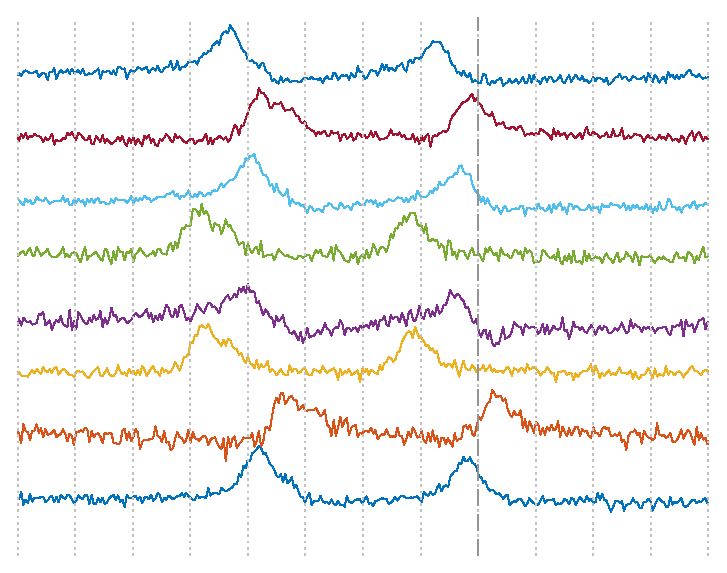
\includegraphics[width=0.95\textwidth, keepaspectratio]{images/samples_transients/8coil_w_phase_w_fshift_cropped.eps}
        \caption{Raw spectral transients}
        \label{subfig:raw transients}        
    \end{subfigure}
    \begin{subfigure}{0.32\textwidth}
        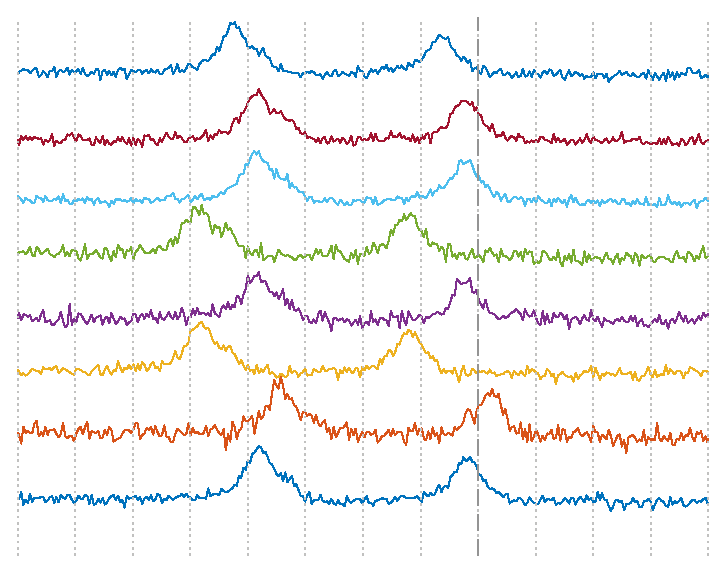
\includegraphics[width=0.95\textwidth, keepaspectratio]{images/samples_transients/8coil_wo_phase_w_fshift_cropped.eps}
        \caption{Phase alignment}
        \label{subfig:phase alignment}        
    \end{subfigure}
    \begin{subfigure}{0.32\textwidth}
        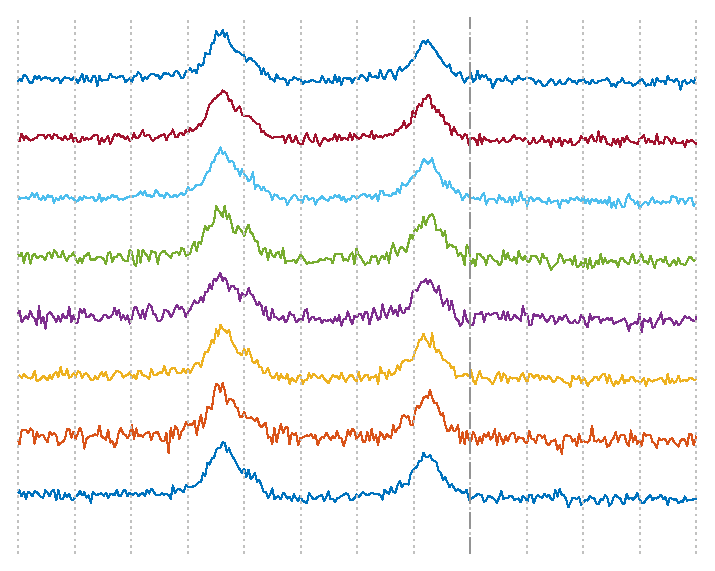
\includegraphics[width=0.95\textwidth, keepaspectratio]{images/samples_transients/8coil_wo_phase_wo_fshift_cropped.eps}
        \caption{Frequency alignment}
        \label{subfig:frequency alignment}        
    \end{subfigure}
    \caption{Examples of 8 simulated coil transients for a 3T GE PRESS sequence with TE=30ms. \ref{subfig:raw transients} shows transients with various SNRs and coil sensitivities along with zero-order phase and frequency offsets. \ref{subfig:phase alignment} shows the transients after phase alignment. \ref{subfig:frequency alignment} shows the transients after frequency alignment. After \ref{subfig:frequency alignment}, the transients can be averaged together and the coil-combined spectrum can then be fitted.}
    \label{fig:simulated transients}
\end{figure}
